\section{生命周期}
在之前的所有权一节,有这么一个函数示例:
\begin{code-block}{rust}
fn first_word(s: &str) -> &str {
    return &s[..];
}

fn copy_ref(s: &str) -> &str {
    // 也可以是&s,为啥?
    return s;
}
\end{code-block}
上述的函数都运行正常。对函数进行改造,改造成下列的样式:
\begin{code-block}{rust}
fn longest(x: &str, y: &str) -> &str {
    if x.len() > y.len() {
        x
    } else {
        y
    }
}
\end{code-block}
即,返回2个字符串当中最长的。如果对这样的代码进行编译,则会出现错误:
\begin{figure}[H]
  \centering
  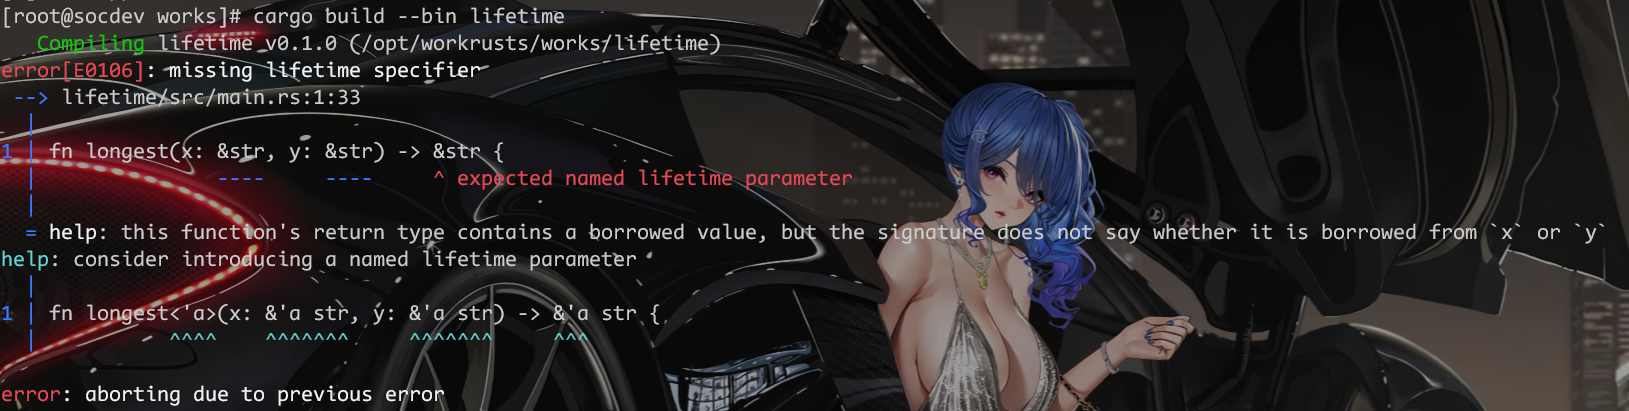
\includegraphics[scale=0.2]{rust_strref_err.png}
  \caption{试图返回多个引用当中的某一个}
  \label{fig:rust_strref_err}
\end{figure}
错误表示,函数应该返回一个有生命周期的命名变量。错误的原因是,Rust编译器无法知道
函数返回的到底是x还是y的引用,无法确定对应的变量的生命周期。

Rust当中,针对引用和借用,有一个特殊的机制:借用检查器,其作用比较作用域来确保所
有的借用都是有效的。
\begin{code-block}{rust}
{
    let r;                      // ---------+-- 'a
    {                            //          |
        let x = 5;             // -+-- 'b  |
        r = &x;                 //  |       |
    }                            // -+       |
    println!("r: {}", r); // ---------+
}
\end{code-block}

其中'a表示变量r原本的作用域(生命周期),'b则表示变量x的有效作用域。进入'b作用域
之后,r变量引用了一个作用域为'b的变量x,当退出'b之后,x失去作用,导致作为x的引用
的r也失去作用,被回收,因此,上述代码无法进行编译:'b的作用范围比'a要小。

为了解决这类的问题,Rust引入了生命周期的操作。生命周期的定义通常使用'+名称的方式
进行定义,表示一个变量或者函数的有效范围,如下:
\begin{code-block}{rust}
&i32        // 引用
&'a i32     // 带有显式生命周期的引用
&'a mut i32 // 带有显式生命周期的可变引用
\end{code-block}
生命周期不仅可以用于变量,同样可以作用与函数和方法上:
\begin{code-block}{rust}
fn main() {
    let string1 = String::from("abcd");
    let string2 = "xyz";

    let res = longest(&string1, string2);
    println!("The result is {}", res);
    println!("The result is {}", res);
}

fn longest<'a>(x: &'a str, y: &'a str) -> &'a str {
    if x.len() > y.len() {
        x
    } else {
        y
    }
}
\end{code-block}
上述代码表示,参数列表当中的所有引用都必须拥有相同的生命周期'a,通过生命周期的限定,
上述代码可以正常编译,并且正常执行。需要注意,如果在参数上使用生命周期,则函数/方法
的前面,则必须加上生命周期,否则会提示参数列表当中的生命周期没有定义。

生命周期同样可以应用于结构体字段定义当中,如下:
\begin{code-block}{rust}
struct ImportantExcerpt<'a> {
    part: &'a str,
}
\end{code-block}

上述结构体的初始化,则可以直接使用字符串的引用进行实现:
\begin{code-block}{rust}
let i = ImportantExcerpt { part: "zhangjl" };
println!("{}", i.part);
\end{code-block}

对于带有生命周期的结构体,在使用的时候,尤其是函数定义和方法定义时,有一些必须
注意的细节:
\begin{outline}[enumerate]
\1 传入外部引用数据模式

使用这种模式,通常情况下,不需要对函数添加生命周期,和普通函数相同。不过,也可以
使用添加生命周期的完整形式:
\begin{code-in-enumerate}{rust}
fn init_struct(source: &str) -> ImportantExcerpt {
    return ImportantExcerpt { part: source };
}

// 使用生命周期的完整形式,实际上是上述函数的完整签名形式
// fn init_struct<'a>(source: &'a str) -> ImportantExcerpt<'a> {
//     return ImportantExcerpt { part: source };
// }

...

// 调用函数
let b = init_struct("luoyan");
\end{code-in-enumerate}
由于上述代码当中,结构体的变量的有效生命周期和外部引用的相同,因此,可以简化生命
周期的使用。

\1 使用函数局部变量

在这种方式下,由于局部引用变量的作用域有限,返回函数之后就不存在了,因此,必须使用
显式的生命周期,而显式的生命周期使用同样有2种形式:
\begin{code-in-enumerate}{rust}
fn init_struct<'a>() -> ImportantExcerpt<'a> {
    return ImportantExcerpt { part: "luoyan"};
}

// 使用静态生命周期,'static表示静态生命周期,为固定关键字
// fn init_struct() -> ImportantExcerpt<'static> {
//     return ImportantExcerpt { part: "luoyan"};
// }
\end{code-in-enumerate}

\1 实现Trait

包含有引用数据类型的结构体,也可以实现各种标准库的Trait。在实现Trait的时候,也
必须使用生命周期:
\begin{code-in-enumerate}{rust}
// 可替换成下面的代码
// impl<'a> fmt::Display for ImportantExcerpt<'a> {
// static可以替换为_
impl fmt::Display for ImportantExcerpt<'static> {
    fn fmt(&self, f: &mut fmt::Formatter) -> fmt::Result {
        write!(f, "{}", self.part)
    }
}
\end{code-in-enumerate}

\1 添加结构体方法

结构体存在引用数据类型,同样要求结构体的方法在实现时需要进行额外的处理,添加生命
周期的使用,同样的,结构体的方法可以使用命名生命周期,也可以使用固定生命周期:
\begin{code-in-enumerate}{rust}
// 使用命名生命周期的结构体方法声明
impl<'a> ImportantExcerpt<'a> {
    fn show(&self) {
        println!("{}", self.part);
    }

    fn reset(&mut self, other: &'a str) {
        self.part = other;
    }

    fn get(&self) -> &str {
        return self.part;
    }
}

// 使用固定生命周期的结构体方法声明
impl ImportantExcerpt<'static> {
    fn show(&self) {
        println!("{}", self.part);
    }

    fn reset(&mut self, other: &'static str) {
        self.part = other;
    }

    fn get(&self) -> &str {
        return self.part;
    }
}
\end{code-in-enumerate}

\end{outline}

在上述的代码当中,很多地方都使用了'static静态生命周期。这是一种特殊的生命周期,
能够存活于整个程序期间,所有的字符串字面值都拥有'static生命周期。但是,并不是
任何情况都建议使用static生命周期。

由于生命周期和泛型以及Trait都非常类似,不可避免的,有可能会遇到几者合用的的情况,
在使用的时候,需要将生命周期与泛型使用,分割开,并且,生命周期应当放在首位。
\begin{code-block}{rust}
fn longest_with_an_announcement<'a, T>(x: &'a str, y: &'a str, ann: T) -> &'a str
    where T: Display
{
    println!("Announcement! {}", ann);
    if x.len() > y.len() {
        x
    } else {
        y
    }
}
\end{code-block}

\section{测试}
Rust的测试与其他语言相同,分为单元测试和集成测试。但不管是单元测试,还是集成测试,
在测试当中,都需要遵循相同的测试规则。在默认的lib类型的crate当中,默认情况下,自动
生成的lib.rs会生成如下的代码:
\begin{code-block}{rust}
#[cfg(test)]
mod tests {
    #[test]
    fn it_works() {
        assert_eq!(2 + 2, 4);
    }
}
\end{code-block}
其中,\#[cfg(test)]表示这是一个测试模块,而\#[test]则表示接下来的函数或者方法是测试
函数,it\_works表示测试的函数/方法名,可以变更为其他的名称。其中,assert!、assert\_eq!
和assert\_ne!这3个宏定义,用于检测运行结果、是否相等/是否不等,比如检测返回值当中
是否包含特定的字符串:
\begin{code-block}{rust}
pub fn greeting(name: &str) -> String {
    format!("Hello {}!", name)
}

#[cfg(test)]
mod tests {
    // 引用暴露的模块代码
    use super::*;

    #[test]
    fn greeting_contains_name() {
        let result = greeting("Carol");
        assert!(result.contains("Carol"));
    }
}
\end{code-block}

如果需要测试panic的代码,则可以使用should\_panic宏进行,该宏表示期望对应的函数在
运行的时候出现panic:
\begin{code-block}{rust}
pub struct Guess {
    value: i32,
}

impl Guess {
    pub fn new(value: i32) -> Guess {
        if value < 1 || value > 100 {
            panic!("Guess value must be between 1 and 100, got {}.", value);
        }

        Guess {
            value
        }
    }
}

#[cfg(test)]
mod tests {
    use super::*;

    #[test]
    #[should_panic]
    fn greater_than_100() {
        Guess::new(200);
    }
}
\end{code-block}
如果测试失败,想在测试结果当中,提示出具体的测试错误信息,则可以添加should\_panic
属性中的expected参数:
\begin{code-block}{rust}
#[cfg(test)]
mod tests {
    use super::*;

    #[test]
    #[should_panic(expected = "Guess value must be between 1 and 100")]
    fn greater_than_100() {
        Guess::new(200);
    }
}
\end{code-block}

运行测试用例时,只需要简单的输入如下的指令即可:
\begin{code-block}{bash}
// 默认并行的方式运行所有的测试用例
cargo test

// 串行的方式运行所有的测试用例
cargo test -- --test-threads=1

// 运行指定的测试用例,可匹配以add开头的所有测试用例
cargo test add
\end{code-block}

需要单独说明的是Rust的集成测试。集成测试通常针对lib型的crate。其测试过程大致如下:
\begin{outline}[enumerate]
\1 创建一个lib,并编写代码

\begin{code-in-enumerate}{bash}
cargo new --lib shared
\end{code-in-enumerate}

\1 在shared的src同级目录下,创建集成测试用例目录:
\begin{code-in-enumerate}{bash}
# 文件夹名称固定为tests
mkdir tests
\end{code-in-enumerate}

\1 在tests下创建集成测试用例
\begin{code-in-enumerate}{bash}
echo > tests/units.rs<<EOF
// 导入的lib名称必须是当前crate的名称
use shared;

#[test]
fn it_adds_two() {
    assert_eq!(4, adder::add_two(2));
}
EOF
\end{code-in-enumerate}
然后执行测试即可。
\end{outline}

\section{Rust的函数式编程}
Rust同样支持函数式编程。相比于其他语言,Rust的函数式编程性能和效率更高。Rust常见的
函数式编程模式包括闭包和迭代器2大类。

\subsection{闭包}
Rust的闭包和Python当中的非常类似,都可以直接读取外部的变量。其定义的形式基本如下:
\begin{code-block}{rust}
let expensive_closure = |num| {
    println!("calculating slowly...");
    num * 10
};

let res = expensive_closure(10);
\end{code-block}
其中两个||表示定义一个闭包,中间的num表示闭包的参数。如果闭包需要处理多个参数,则
应该改写为:
\begin{code-block}{rust}
let expensive_closure = |num1, num2| {
    num1 * num2
};
\end{code-block}

从实际的使用当中可以看到,Rust的闭包实际上就是一个匿名函数,在Rust当中,函数都有
参数类型/返回值的声明,但是,在上述的代码当中,却没有看到相关的定义和声明。这是
因为Rust的闭包通常很短,并只关联于小范围的上下文而非任意情境。在这些有限制的上下
文中,编译器有能力可靠的推断参数和返回值的类型,如同能够推断大部分变量的类型一样。
不过,不注明参数/返回类型,有可能出现一种迷惑性的使用:即无法传入正确的数据类型,
如下:
\begin{code-block}{rust}
let example_closure = |x| x;

let s = example_closure(String::from("hello"));
let n = example_closure(5);
\end{code-block}
按照上述代码的定义,example\_closure只是将输入参数原封不动的返回给调用者,第1次
调用时,编译器会将该闭包推断为输入/输出为字符串类型,然后这些类型信息会被锁定到
该闭包当中。后续再传入数值,由于闭包的类型已经锁定,要求传入字符串,但实际传入的
是数值,结果就会导致上述代码出现错误:
\begin{figure}[H]
  \centering
  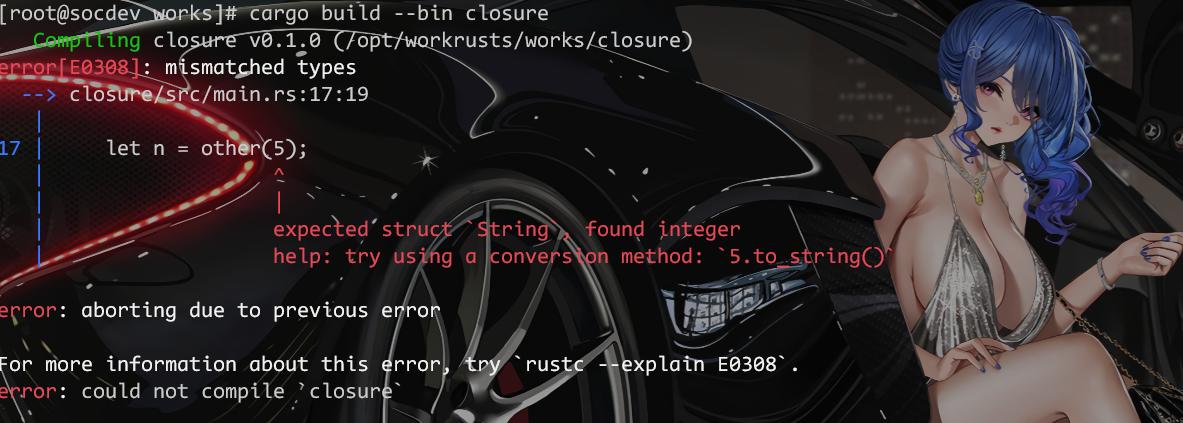
\includegraphics[width=\linewidth]{rust_closure_diffrent_type.png}
  \caption{试图处理不同数据类型的闭包}
  \label{fig:rust_closure_diffrent}
\end{figure}

闭包的完整定义(包括类型)则如下:
\begin{code-block}{rust}
let live_closure = |num: i32| -> (i32, i32) {
    println!("calculating slowly...");
    thread::sleep(Duration::from_secs(2));
    (num * 10, num * 20)
    // 或者修改为return语句
    // return (num*10, num*20);
    // 如果不需要返回值,则最后一定要添加;
};
\end{code-block}
